Krystall-oscillatorer er teknologien bak mange klokker og mesteparten av
teknologien vi bruker i dag.
De fungerer ved piezoelektrisk effekt.
Det vil si at strøm påført elementet medfører mekanisk deformasjon.
Tilsvarende vil et mekanisk trykk på elementet generere elektrisk spenning.
Resonansfrekvensen bestemmes av krystallets fysiske størrelse.

Fordeler:
\begin{itemize}
  \item Stabil
  \item Høy frekvens
  \item Billig
  \item Lavt energikrav
\end{itemize}

\begin{circuitikz} \draw
%Bottom
(1,0) to[short, o-] (1,1)
(0,1) -- (2,1)

%Left
(0,1) to[R, l=$R$] (0,3)
      to[C, l=$C$] (0,5)
      to[L, l=$L$] (0,7)

%Right
(2,7) to[C, l=$C_m$] (2,1)

%Top
(0,7) -- (2,7)
(1,7) to[short, -o] (1,8)
      ;
\end{circuitikz}

Krystallet har to resonansfrekvenser avhengig av om man ser på serieresonansen
av $RCL$ eller parallellresosansen med $RL$ og $C_M$.

\begin{figure}[H]
  \caption{Resonansfrekvens for paralell og serie}
  \centering
  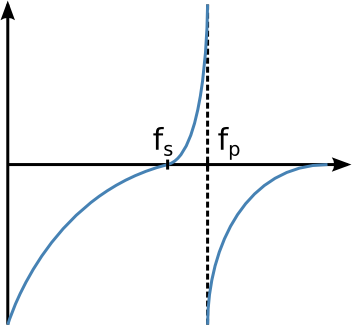
\includegraphics[width=0.5\textwidth]{./img/krystallresonans}
\end{figure}
